\documentclass{article}

\usepackage[pdftex]{hyperref}
\usepackage{graphicx}
\usepackage{listings}

\addtolength{\hoffset}{-2cm}
\addtolength{\textwidth}{4cm}
\addtolength{\voffset}{-2cm}
\addtolength{\textheight}{3cm}

\lstset{language=c,columns=fullflexible,identifierstyle=\itshape} %,literate={&*&}{{$\mathrm{{\&}{*}{\&}}$}}1}

\newtheorem{exercise}{Exercise}

\title{The VeriFast Program Verifier: A Tutorial\\
---Under Construction---}

\author{Bart Jacobs \and Jan Smans \and Frank Piessens}

\begin{document}

\maketitle

\section{Introduction}

VeriFast is a program verification tool for verifying certain
correctness properties of single-threaded and multithreaded C
programs. The tool reads a C program consisting of one or more
.c source code files (plus any .h header files referenced from
these .c files) and reports either ``0 errors found'' or
indicates the location of a potential error. If the tool
reports ``0 errors found'', this means\footnote{There are a few
known reasons (known as \emph{unsoundnesses}) why the tool may
sometimes incorrectly report ``0 errors found''; see the
``Known unsoundnesses'' section in the Reference Manual. There
may also be unknown unsoundnesses.} that the program
\begin{itemize}
\item does not perform illegal memory accesses, such as
    reading or writing a struct instance field after the
    struct instance has been freed, and
\item does not include a certain type of concurrency errors
    known as \emph{data races}, i.e. unsynchronized
    conflicting accesses of the same field by multiple
    threads. Accesses are considered conflicting if at
    least one of them is a write access. And
\item complies with function preconditions and
    postconditions specified by the programmer in the form
    of special comments (known as \emph{annotations}) in
    the source code.
\end{itemize}

We will now proceed to introduce the tool's features step by
step. To try the examples and exercises in this tutorial
yourself, please download the release from the VeriFast website
at
\begin{center}
\texttt{http://www.cs.kuleuven.be/\symbol{126}bartj/verifast/}
\end{center}
. You will find a command-line version of the tool
(\texttt{verifast.exe}), and a version that presents a
graphical user interface (\texttt{vfide.exe}). The example C
programs used in this tutorial are in the \texttt{tutorial}
directory.

\section{Example: illegal\_access.c}

Please start \texttt{vfide.exe} with the
\texttt{illegal\_access.c} program. The program will be shown
in the VeriFast IDE. To verify the program, choose the
\textbf{Verify program} command in the \textbf{Verify} menu,
press the \textbf{Play} toolbar button, or press F5. You will
see something like this:
\begin{center}
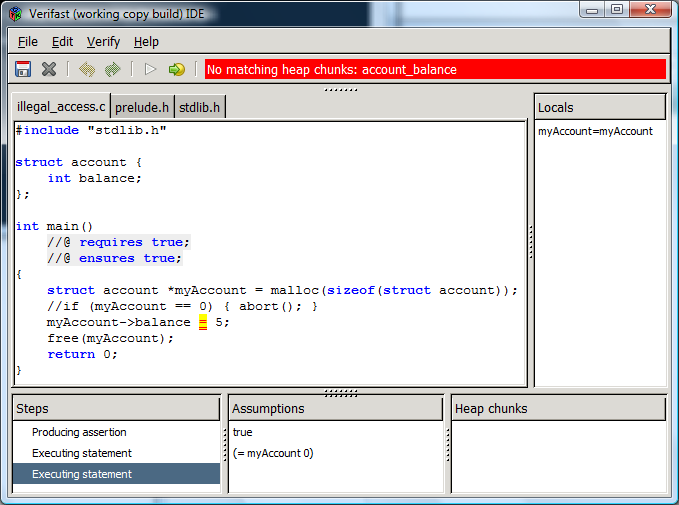
\includegraphics[width=7cm]{illegal_access.png}
\end{center}
The program attempts to access a field of a struct instance
allocated using $\mathit{malloc}$. However, if there is
insufficient memory, $\mathit{malloc}$ returns zero and no
memory is allocated. VeriFast detects the illegal memory access
that happens in this case. Notice the following GUI elements:
\begin{itemize}
\item The erroneous program element is displayed in a red
    color with a double underline.
\item The error message states: ``No matching heap chunks:
    account\_balance''. Indeed, in the scenario where there
    is insufficient memory, the memory location (or
    \emph{heap chunk}) that the program attempts to access
    is not accessible to the program.
    $\mathsf{account\_balance}$ is the type of heap chunk
    that represents the $\mathsf{balance}$ field of an
    $\mathsf{account}$ struct instance.
\item The assignment statement is shown on a yellow
    background. This is because the assignment statement is
    the \emph{current step}. VeriFast verifies each
    function by stepping through it, while keeping track of
    a symbolic representation of the relevant program
    state. You can inspect the symbolic state at each step
    by selecting the step in the Steps pane in the lower
    left corner of the VeriFast window. The program element
    corresponding to the current step is shown on a yellow
    background. The symbolic state consists of the
    \emph{path condition}, shown in the Assumptions pane;
    the \emph{symbolic heap}, shown in the Heap chunks
    pane; and the \emph{symbolic store}, shown in the
    Locals pane.
\end{itemize}

To correct the error, uncomment the commented statement. Now
press F5 again. The program now verifies and no symbolic
execution path is shown in the Steps pane.

To inspect the symbolic execution of the $\mathsf{main}$
function anyway, place the cursor on the last line (i.e., on
the brace that closes the function body) and choose the
\textbf{Run to cursor} command from the \textbf{Verify} menu,
press the \textbf{Run to cursor} toolbar button, or press
Ctrl+F5.
\begin{center}
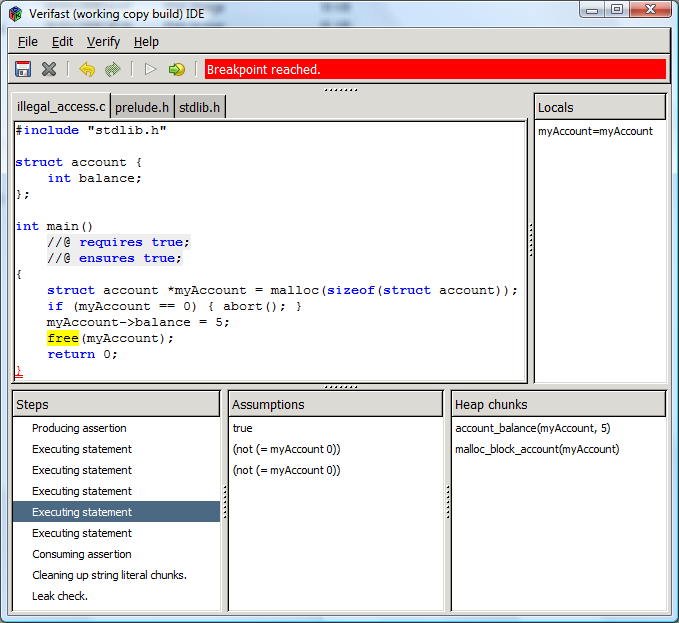
\includegraphics[width=7cm]{illegal_access2.png}
\end{center}
Running to the cursor means showing an execution path that
reaches the cursor. In general, there may be multiple such
paths; in that case, the first such path is chosen (in the
order on paths induced by the order on branches induced by the
program text). In the example, there is only one path.

To understand how VeriFast tracks the state of memory, select
the fifth step in the Steps pane, as in the figure. The
$\mathit{free}$ statement is the next statement to be executed.
In this step, the symbolic heap contains two heap chunks:
$\mathsf{account\_balance}(\mathsf{myAccount}, 5)$ and
$\mathsf{malloc\_block\_account}(\mathsf{myAccount})$. The
first heap chunk denotes the fact that the $\mathsf{balance}$
field of the $\mathsf{account}$ struct instance at address
$\mathsf{myAccount}$ is accessible to the program, and has
value 5. The second heap chunk denotes the fact that the
program has permission to de-allocate the memory block at
address $\mathsf{myAccount}$. If you select the next step, you
notice that the $\mathit{free}$ statement removes both heap
chunks from the symbolic heap. Indeed, de-allocating the struct
instance removes both the permission to access the struct
instance's field, and the permission to free the struct
instance. This prevents illegal memory accesses and double free
errors.

\section{Functions and Contracts}

We continue to play with the example of the previous section.
The example currently consists of only one function: the main
function. Let's add another function. Write a function
$\mathsf{account\_set\_balance}$ that takes the address of an
$\mathsf{account}$ struct instance and a integer amount, and
assigns this amount to the struct instance's $\mathsf{balance}$
field. Then replace the field assignment in the main function
with a call to this function. We now have the following
program:

\begin{lstlisting}
#include "stdlib.h"

struct account {
    int balance;
};

void account_set_balance(struct account *myAccount, int newBalance)
{
    myAccount->balance = newBalance;
}

int main()
    //@ requires true;
    //@ ensures true;
{
    struct account *myAccount = malloc(sizeof(struct account));
    if (myAccount == 0) { abort(); }
    account_set_balance(myAccount, 5);
    free(myAccount);
    return 0;
}
\end{lstlisting}

If we try to verify the new program, VeriFast complains that
the new function has no contract. Indeed, VeriFast verifies
each function separately, so it needs a precondition and a
postcondition for each function to describe the initial and
final state of calls of the function.

Add the same contract that the main function has:
\begin{lstlisting}
void account_set_balance(struct account *myAccount, int newBalance)
    //@ requires true;
    //@ ensures true;
\end{lstlisting}
Notice that contracts, like all VeriFast annotations, are in
comments, so that the C compiler ignores them. VeriFast also
ignores comments, except the ones that are marked with an at
(\verb|@|) sign.

VeriFast now no longer complains about missing contracts.
However, it now complains that the field assignment in the body
of $\mathsf{account\_set\_balance}$ cannot be verified because
the symbolic heap does not contain a heap chunk that grants
permission to access this field. To fix this, we need to
specify in the function's precondition that the function
requires permission to access the $\mathsf{balance}$ field of
the $\mathsf{account}$ struct instance at address
$\mathsf{myAccount}$. We achieve this simply by mentioning the
heap chunk in the precondition:
\begin{lstlisting}
void account_set_balance(struct account *myAccount, int newBalance)
    //@ requires account_balance(myAccount, _);
    //@ ensures true;
\end{lstlisting}
Notice that we use an underscore in the position where the
value of the field belongs. This indicates that we do not care
about the old value of the field when the function is
called.\footnote{VeriFast also supports a more concise syntax
for field chunks. For example,
\lstinline!account_balance(myAccount, _)! can also be written as
\lstinline!myAccount->balance |-> _!.}

VeriFast now highlights the brace that closes the body of the
function. This means we successfully verified the field
assignment. However, VeriFast now complains that the function
leaks heap chunks. For now, let's simply work around this error
message by inserting a $\mathbf{leak}$ command, which indicates
that we're happy to leak this heap chunk. We will come back to
this later.
\begin{lstlisting}
void account_set_balance(struct account *myAccount, int newBalance)
    //@ requires account_balance(myAccount, _);
    //@ ensures true;
{
    myAccount->balance = newBalance;
    //@ leak account_balance(myAccount, _);
}
\end{lstlisting}

Function $\mathsf{account\_set\_balance}$ now verifies, and
VeriFast attempts to verify function $\mathsf{main}$. It
complains that it cannot free the $\mathsf{account}$ struct
instance because it does not have permission to access the
$\mathsf{balance}$ field. Indeed, the symbolic heap contains
the $\mathsf{malloc\_block\_account}$ chunk but not the
$\mathsf{account\_balance}$ chunk. What happened to it? Let's
find out by stepping through the symbolic execution path.
Select the third step. The $\mathsf{malloc}$ statement is about
to be executed and the symbolic heap is empty. Select the next
step. The $\mathsf{malloc}$ statement has added the
$\mathsf{account\_balance}$ chunk and the
$\mathsf{malloc\_block\_account}$ chunk. The if statement has
no effect.

We then arrive at the call of $\mathsf{account\_set\_balance}$.
You will notice that this execution step has two sub-steps,
labeled ``Consuming assertion'' and ``Producing assertion''.
The verification of a function call consists of
\emph{consuming} the function's precondition and then
\emph{producing} the function's postcondition. The precondition
and the postcondition are \emph{assertions}, i.e., expressions
that may include heap chunks in addition to ordinary logic.
Consuming the precondition means passing the heap chunks
required by the function to the function, thus removing them
from the symbolic heap. Producing the postcondition means
receiving the heap chunks offered by the function when it
returns, thus adding them to the symbolic heap.

Selecting the ``Consuming assertion'' step changes the layout
of the VeriFast window.
\begin{center}
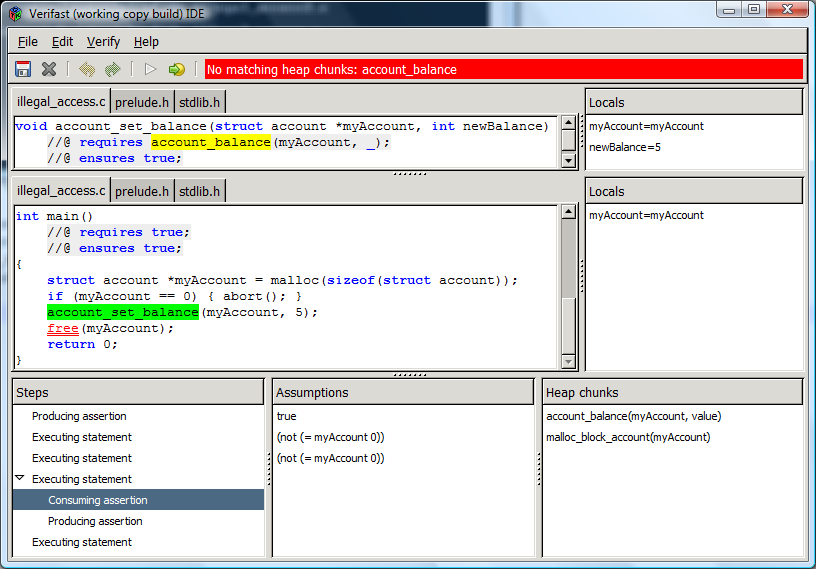
\includegraphics[width=7cm]{illegal_access3.png}
\end{center}
The source code pane is split into two
parts. The upper part is used to display the contract of the
function being called, while the lower part is used to display
the function being verified. (Since in this example the
function being called is so close to the function being
verified, it is likely to be shown in the lower part as well.)
The call being verified is shown on a green background. The
part of the contract being consumed or produced is shown on a
yellow background. If you move from the ``Consuming assertion''
step to the ``Producing assertion'' step, you notice that the
``Consuming assertion'' step removes the
$\mathsf{account\_balance}$ chunk from the symbolic heap.
Conceptually, it is now in use by the
$\mathsf{account\_set\_balance}$ function while the
$\mathsf{main}$ function waits for this function to return.
Since function $\mathsf{account\_set\_balance}$'s postcondition
does not mention any heap chunks, the ``Producing assertion''
step does not add anything to the symbolic heap.

It is now clear why VeriFast complained that
$\mathsf{account\_set\_balance}$ leaked heap chunks: since the
function did not return the $\mathsf{account\_balance}$ chunk
to its caller, the chunk was lost and the field could never be
accessed again. VeriFast considers this an error since it is
usually not the intention of the programmer; furthermore, if
too many memory locations are leaked, the program will run out
of memory.

It is now also clear how to fix the error: we must specify in
the postcondition of function $\mathsf{account\_set\_balance}$
that the function must hand back the
$\mathsf{account\_balance}$ chunk to its caller.
\begin{lstlisting}
void account_set_balance(struct account *myAccount, int newBalance)
    //@ requires account_balance(myAccount, _);
    //@ ensures account_balance(myAccount, newBalance);
{
    myAccount->balance = newBalance;
}
\end{lstlisting}
 This
eliminates the leak error message and the error at the
$\mathit{free}$ statement. The program now verifies. Notice
that we refer to the $\mathsf{newBalance}$ parameter in the
position where the value of the field belongs; this means that
the value of the field when the function returns must be equal
to the value of the parameter.

\begin{exercise}\label{exercise:account1}
Now factor out the creation and the disposal of the
$\mathsf{account}$ struct instance into separate functions as
well. The creation function should initialize the balance to
zero. Note: if you need to mention multiple heap chunks in an
assertion, separate them using the \emph{separate conjunction}
\lstinline!&*&! (ampersand-star-ampersand). Also, you can refer
to a function's return value in its postcondition by the name
\lstinline!result!.
\end{exercise}

\section{Patterns}

Now, let's add a function that returns the current balance, and
let's test it in the main function. Here's our first attempt:

\begin{lstlisting}
int account_get_balance(struct account *myAccount)
    //@ requires account_balance(myAccount, _);
    //@ ensures account_balance(myAccount, _);
{
    return myAccount->balance;
}

int main()
    //@ requires true;
    //@ ensures true;
{
    struct account *myAccount = create_account();
    account_set_balance(myAccount, 5);
    int b = account_get_balance(myAccount);
    assert(b == 5);
    account_dispose(myAccount);
    return 0;
}
\end{lstlisting}

The new function verifies successfully, but VeriFast complains
that it cannot prove the condition \lstinline!b == 5!. When
VeriFast is asked to check a condition, it first translates the
condition to a logical formula, by replacing each variable by
its symbolic value. We can see in the symbolic store, displayed
in the Locals pane, that the symbolic value of variable
$\mathsf{b}$ is the logical symbol $\mathsf{b}$. Therefore, the
resulting logical formula is \lstinline!b == 5!. VeriFast then
attempts to derive this formula from the \emph{path condition},
i.e., the formulae shown in the Assumptions pane. Since the
only assumption in this case is \lstinline!true!, VeriFast
cannot prove the condition.

The problem is that the postcondition of function
$\mathsf{account\_get\_balance}$ does not specify the
function's return value. It does not state that the return
value is equal to the value of the $\mathsf{balance}$ field
when the function is called. To fix this, we need to be able to
assign a name to the value of the balance field when the
function is called. We can do so by replacing the underscore in
the precondition by the \emph{pattern} \lstinline!?theBalance!.
This causes the name \lstinline!theBalance! to be bound to the
value of the $\mathsf{balance}$ field. We can then use this
name in the postcondition to specify the return value using an
equality condition. A function's return value is available in
the function's postcondition under the name \lstinline!result!.
Logical conditions and heap chunks in an assertion must be
separated using the separating conjunction \lstinline!&*&!.
\begin{lstlisting}
int account_get_balance(struct account *myAccount)
    //@ requires account_balance(myAccount, ?theBalance);
    //@ ensures account_balance(myAccount, theBalance) &*& result == theBalance;
{
    return myAccount->balance;
}
\end{lstlisting}
Notice that we use the \lstinline!theBalance! name also to
specify that the function does not modify the value of the
$\mathsf{balance}$ field, by using the name again in the field
value position in the postcondition.

The program now verifies. Indeed, if we use the \textbf{Run to
cursor} command to run to the $\mathit{assert}$ statement, we
see that the assumption \lstinline!(= b 5)! has appeared in the
Assumptions pane. If we step up, we see that it was added when
the equality condition in function
$\mathsf{account\_get\_balance}$'s postcondition was produced.
If we step up further, we see that the variable
\lstinline!theBalance! was added to the upper Locals pane when
the field chunk assertion was consumed, and bound to value 5.
It was bound to value 5 because that was the value found in the
symbolic heap. When verifying a function call, the upper Locals
pane is used to evaluate the contract of the function being
called. It initially contains the bindings of the function's
parameters to the arguments specified in the call; additional
bindings appear as patterns are encountered in the contract.
The assumption \lstinline!(= b 5)! is the logical formula
obtained by evaluating the equality condition %
\lstinline!result == theBalance! under the symbolic store shown
in the upper Locals pane.

\begin{exercise}\label{exercise:account2}
Add a function that deposits a given amount into an account.
Verify the following \lstinline!main! function.
\begin{lstlisting}
int main()
    //@ requires true;
    //@ ensures true;
{
    struct account *myAccount = create_account();
    account_set_balance(myAccount, 5);
    account_deposit(myAccount, 10);
    int b = account_get_balance(myAccount);
    assert(b == 15);
    account_dispose(myAccount);
    return 0;
}
\end{lstlisting}
Note: VeriFast checks for arithmetic overflow. For now, disable
this check in the \textbf{Verify} menu.
\end{exercise}

\begin{exercise}\label{exercise:account3}
Add a field \lstinline!limit! to struct \lstinline!account!.
The limit is specified at creation time. Further add a function
to withdraw a given amount from an account. The function must
not withdraw more than allowed by the limit. The function
returns the amount actually withdrawn as its return value. You
will need to use C's conditional expressions
\lstinline!condition ? value1 : value2!. Remove function
\lstinline!account_set_balance!. Use the shorthand notation for
field chunks: \lstinline!myAccount->balance |-> value!. Verify
the following \lstinline!main! function.
\begin{lstlisting}
int main()
    //@ requires true;
    //@ ensures true;
{
    struct account *myAccount = create_account(-100);
    account_deposit(myAccount, 200);
    int w1 = account_withdraw(myAccount, 50);
    assert(w1 == 50);
    int b1 = account_get_balance(myAccount);
    assert(b1 == 150);
    int w2 = account_withdraw(myAccount, 300);
    assert(w2 == 250);
    int b2 = account_get_balance(myAccount);
    assert(b2 == -100);
    account_dispose(myAccount);
    return 0;
}
\end{lstlisting}
\end{exercise}

\section{Predicates}

We continue with the program obtained in
Exercise~\ref{exercise:account3}. We observe that the contracts
are becoming rather long. Furthermore, if we consider the
account ``class'' and the main function to be in different
modules, then the internal implementation details of the
account module are exposed to the main function. We can achieve
more concise contracts as well as information hiding by
introducing a \emph{predicate} to describe an
$\mathsf{account}$ struct instance in the function contracts.
\begin{lstlisting}
/*@
predicate account_pred(struct account *myAccount, int theLimit, int theBalance) =
    myAccount->limit |-> theLimit &*& myAccount->balance |-> theBalance
    &*& malloc_block_account(myAccount);
@*/
\end{lstlisting}
A predicate is a named, parameterized assertion. Furthermore, it introduces a new type of heap chunk.
An \lstinline!account_pred! heap chunk bundles an \lstinline!account_limit! heap chunk, an \lstinline!account_balance! heap chunk,
and a \lstinline!malloc_block_account! heap chunk into one.

Let's use this predicate to rewrite the contract of the deposit function. Here's a first attempt:
\begin{lstlisting}
void account_deposit(struct account *myAccount, int amount)
    //@ requires account_pred(myAccount, ?limit, ?balance) &*& 0 <= amount;
    //@ ensures account_pred(myAccount, limit, balance + amount);
{
    myAccount->balance += amount;
}
\end{lstlisting}
This function does not verify. The update of the
\lstinline!balance! field cannot be verified since there is no
\lstinline!account_balance! heap chunk in the symbolic heap.
There is only a \lstinline!account_pred! heap chunk. The
\lstinline!account_pred! heap chunk encapsulates the
\lstinline!account_balance! heap chunk, but VeriFast does not
``un-bundle'' the \lstinline!account_pred! predicate
automatically. We must instruct VeriFast to un-bundle predicate
heap chunks by inserting an \lstinline!open! ghost statement:
\begin{lstlisting}
void account_deposit(struct account *myAccount, int amount)
    //@ requires account_pred(myAccount, ?limit, ?balance) &*& 0 <= amount;
    //@ ensures account_pred(myAccount, limit, balance + amount);
{
    //@ open account_pred(myAccount, limit, balance);
    myAccount->balance += amount;
}
\end{lstlisting}
The assignment now verifies, but now VeriFast is stuck at the
postcondition. It complains that it cannot find the
\lstinline!account_pred! heap chunk that it is supposed to hand
back to the function's caller. The \lstinline!account_pred!
chunk's constituent chunks are present in the symbolic heap,
but VeriFast does not automatically bundle them up into an
\lstinline!account_pred! chunk. We must instruct VeriFast to do
so using a \lstinline!close! ghost statement:
\begin{lstlisting}
void account_deposit(struct account *myAccount, int amount)
    //@ requires account_pred(myAccount, ?limit, ?balance) &*& 0 <= amount;
    //@ ensures account_pred(myAccount, limit, balance + amount);
{
    //@ open account_pred(myAccount, limit, balance);
    myAccount->balance += amount;
    //@ close account_pred(myAccount, limit, balance + amount);
}
\end{lstlisting}
The function now verifies. However, the main function does not,
since the call of \lstinline!account_deposit! expects an
\lstinline!account_pred! heap chunk.

\begin{exercise}\label{exercise:predicates}
Rewrite the remaining contracts using the
\lstinline!account_pred! predicate. Insert \lstinline!open! and
\lstinline!close! statements as necessary.
\end{exercise}

\section{Recursive Predicates}

In the previous section, we introduced predicates for the sake
of conciseness and information hiding. However, there is an
even more compelling need for predicates: they are the only way
you can describe unbounded-size data structures in VeriFast.
Indeed, in the absence of predicates, the number of memory
locations described by an assertion is linear in the length of
the assertion. This limitation can be overcome through the use
of recursive predicates, i.e., predicates that invoke
themselves.

\begin{exercise}\label{exercise:stack}
Implement a stack of integers using a singly linked list data
structure: implement functions \lstinline!create_stack!,
\lstinline!stack_push!, \lstinline!stack_pop!, and
\lstinline!stack_dispose!. In order to be able to specify the
precondition of \lstinline!stack_pop!, your predicate will need
to have a parameter that specifies the number of elements in
the stack. Function \lstinline!stack_dispose! may be called
only on an empty stack. Do not attempt to specify the contents
of the stack; this is not possible with the annotation elements
we have seen. You will need to use conditional assertions:
\lstinline!condition ? assertion1 : assertion2!. Note: VeriFast
does not allow the use of field dereferences in
\lstinline!open! statements. If you want to use the value of a
field in an \lstinline!open! statement, you must first store
the value in a local variable. Verify the following main
function:
\end{exercise}
\begin{lstlisting}
int main()
    //@ requires true;
    //@ ensures true;
{
    struct stack *s = create_stack();
    stack_push(s, 10);
    stack_push(s, 20);
    stack_pop(s);
    stack_pop(s);
    stack_dispose(s);
    return 0;
}
\end{lstlisting}

Now, let's extend the solution to Exercise~\ref{exercise:stack}
on page~\pageref{solution:stack} with a
\lstinline!stack_is_empty! function. Recall the predicate
definitions:
\begin{lstlisting}
predicate nodes(struct node *node, int count) =
    node == 0 ?
        count == 0
    :
        0 < count
        &*& node->next |-> ?next &*& node->value |-> ?value
        &*& malloc_block_node(node) &*& nodes(next, count - 1);

predicate stack(struct stack *stack, int count) =
    stack->head |-> ?head &*& malloc_block_stack(stack) &*& 0 <= count &*& nodes(head, count);
\end{lstlisting}

Here's a first stab at a \lstinline!stack_is_empty! function:
\begin{lstlisting}
bool stack_is_empty(struct stack *stack)
    //@ requires stack(stack, ?count);
    //@ ensures stack(stack, count) &*& result == (count == 0);
{
    //@ open stack(stack, count);
    bool result = stack->head == 0;
    //@ close stack(stack, count);
    return result;
}
\end{lstlisting}
The function does not verify. VeriFast complains that it cannot
prove the condition \lstinline!result == (count == 0)! in the
postcondition. Indeed, if we look at the assumptions in the
Assumptions pane, they are insufficient to prove this
condition. The problem is that the relationship between the
value of the head pointer and the number of nodes is hidden
inside the \lstinline!nodes! predicate. We need to open the
predicate, so that the information is added to the assumptions.
Of course, we then need to close it again so that we can close
the \lstinline!stack! predicate.
\begin{lstlisting}
bool stack_is_empty(struct stack *stack)
    //@ requires stack(stack, ?count);
    //@ ensures stack(stack, count) &*& result == (count == 0);
{
    //@ open stack(stack, count);
    struct node *head = stack->head;
    //@ open nodes(head, count);
    bool result = stack->head == 0;
    //@ close nodes(head, count);
    //@ close stack(stack, count);
    return result;
}
\end{lstlisting}
The function now verifies. What happens exactly is the
following. When VeriFast executes the open statement, it
produces the conditional assertion in the body of the
\lstinline!nodes! predicate. This causes it to perform a
\emph{case split}. This means that the rest of the function is
verified twice: once under the assumption that the condition is
true, and once under the assumption that the condition is
false. In other words, the execution path splits into two
execution paths, or two \emph{branches}. On both branches, the
postcondition can now be proved easily: on the first branch, we
get the assumptions \lstinline!head == 0! and %
\lstinline!count == 0!, and on the second branch we get
\lstinline$head != 0$ and \lstinline$0 < count$.

\begin{exercise}\label{exercise:stack2}
Modify function \lstinline!stack_dispose! so that it works even
if the stack still contains some elements. Use a recursive
helper function.\footnote{Warning: VeriFast does not verify
termination; it does not complain about infinite recursion or
infinite loops. That is still your own responsibility.}
\end{exercise}

Notice that VeriFast performs a case split when verifying an
\lstinline!if! statement.

\begin{exercise}\label{exercise:stack4}
Add a function \lstinline!stack_get_sum! that returns the sum
of the values of the elements on the stack. Use a recursive
helper function. The contract need not specify the return value
(since we did not see how to do that yet).
\end{exercise}

\section{Loops}

In Exercise~\ref{exercise:stack2}, we implemented
\lstinline!stack_dispose! using a recursive function. However,
this is not an optimal implementation. If our data structure
contains very many elements, we may create too many activation
records and overflow the call stack. It is more optimal to
implement the function using a loop. Here's a first attempt:
\begin{lstlisting}
void stack_dispose(struct stack *stack)
    //@ requires stack(stack, _);
    //@ ensures true;
{
    //@ open stack(stack, _);
    struct node *n = stack->head;
    while (n != 0)
    {
        //@ open nodes(n, _);
        struct node *next = n->next;
        free(n);
        n = next;
    }
    //@ open nodes(0, _);
    free(stack);
}
\end{lstlisting}
This function does not verify. VeriFast complains at the loop
because the loop does not specify a loop invariant. VeriFast
needs a loop invariant so that it can verify an arbitrary
sequence of loop iterations by verifying the loop body once,
starting from a symbolic state that represents the start of an
arbitrary loop iteration (not just the first iteration).

Specifically, VeriFast verifies a loop as follows:
\begin{itemize}
\item First, it consumes the loop invariant.
\item Then, it removes the remaining heap chunks from the
    heap (but it remembers them).
\item Then, it assigns a fresh logical symbol to each local
    variable that is modified in the loop body.
\item Then, it produces the loop invariant.
\item Then, it performs a case split on the loop condition:
    \begin{itemize}
    \item If the condition is true:
    \begin{itemize}
    \item It verifies the loop body,
    \item then it consumes the loop invariant,
    \item and then finally it checks for leaks.
        After this step this execution path is
        finished.
    \end{itemize}
    \item If the condition is false, VeriFast puts the
        heap chunks that were removed in Step 2 back
        into the heap, and then verification continues
        after the loop.
    \end{itemize}
\end{itemize}
Notice that this means that the loop can access only those heap
chunks that are mentioned in the loop invariant.

The correct loop invariant for the above function is as
follows:
\begin{lstlisting}
void stack_dispose(struct stack *stack)
    //@ requires stack(stack, _);
    //@ ensures true;
{
    //@ open stack(stack, _);
    struct node *n = stack->head;
    while (n != 0)
        //@ invariant nodes(n, _);
    {
        //@ open nodes(n, _);
        struct node *next = n->next;
        free(n);
        n = next;
    }
    //@ open nodes(0, _);
    free(stack);
}
\end{lstlisting}

You can inspect the first branch of the execution of the loop
by placing the cursor at the closing brace of the loop body and
choosing the \textbf{Run to cursor} command. Find the
\textit{Executing statement} step for the \lstinline!while!
statement. Notice that this step is followed by a
\textit{Producing assertion} step and a \textit{Consuming
assertion} step. Notice that between these two steps, the value
of variable \lstinline!n! changes from \lstinline!head! to
\lstinline!n!, and all chunks are removed from the symbolic
heap. Further notice that in the next step, the assumption
\lstinline!(not (= n 0))! is added to the Assumptions pane.

You can inspect the second branch of the execution of the loop
by placing the cursor at the closing brace of the function body
and choosing the \textbf{Run to cursor} command. Notice that
the same things happen as in the first branch, except that the
loop body is not executed, and the assumption %
\lstinline!(= n 0)! is added to the Assumptions pane.

\begin{exercise}\label{exercise:stack3}
Specify and implement function \lstinline!stack_popn!, which
pops a given number of elements from the stack (and returns
\lstinline!void!). You may call \lstinline!stack_pop!
internally. Use a \lstinline!while! loop. Notice that your loop
invariant must not only enable verification of the loop body,
but must also maintain the relationship between the current
state and the initial state, sufficiently to prove the
postcondition. This often means that you should not overwrite
the function parameter values, since you typically need the
original values in the loop invariant.
\end{exercise}

\section{Inductive Datatypes}\label{section:datatypes}

Let's return to our initial annotated stack implementation (the
solution to Exercise~\ref{exercise:stack}). The annotations do
not specify full functional correctness. In particular, the
contract of function \lstinline!stack_pop! does not specify the
function's return value. As a result, using these annotations,
we cannot verify the following main function:
\begin{lstlisting}
int main()
    //@ requires true;
    //@ ensures true;
{
    struct stack *s = create_stack();
    stack_push(s, 10);
    stack_push(s, 20);
    int result1 = stack_pop(s);
    assert(result1 == 20);
    int result2 = stack_pop(s);
    assert(result2 == 10);
    stack_dispose(s);
    return 0;
}
\end{lstlisting}

In order to verify this main function, instead of tracking just
the number of elements in the stack, we need to track the
values of the elements as well. In other words, we need to
track the precise sequence of elements currently stored by the
stack. We can represent a sequence of integers using an
\emph{inductive datatype} \lstinline!ints!:
\begin{lstlisting}
inductive ints = ints_nil | ints_cons(int, ints);
\end{lstlisting}
This declaration declares a type \lstinline!ints! with two
\emph{constructors} \lstinline!ints_nil! and
\lstinline!ints_cons!. \lstinline!ints_nil! represents the
empty sequence. \lstinline!ints_cons! constructs a nonempty
sequence given the \emph{head} (the first element) and the
\emph{tail} (the remaining elements). For example, the sequence
1,2,3 can be written as
\begin{lstlisting}
ints_cons(1, ints_cons(2, ints_cons(3, ints_nil)))
\end{lstlisting}

\begin{exercise}\label{exercise:stack4}
Replace the \lstinline!count! parameter of the
\lstinline!nodes! and \lstinline!stack! predicates with a
\lstinline!values! parameter of type \lstinline!ints! and
update the predicate bodies. Further update the functions
\lstinline!create_stack!, \lstinline!stack_push!, and
\lstinline!stack_dispose!.
\end{exercise}

How should we update the annotations for function
\lstinline!stack_pop!? We need to refer to the tail of the
current sequence in the postcondition and in the close
statement. Furthermore, in order to specify the return value,
we need to refer to the head of the current sequence. We can do
so using \emph{fixpoint functions}:
\begin{lstlisting}
fixpoint int ints_head(ints values) {
    switch (values) {
        case ints_nil: return 0;
        case ints_cons(value, values0): return value;
    }
}

fixpoint ints ints_tail(ints values) {
    switch (values) {
        case ints_nil: return ints_nil;
        case ints_cons(value, values0): return values0;
    }
}
\end{lstlisting}
Notice that we can use switch statements on inductive
datatypes. There must be exactly one case for each constructor.
In a case for a constructor that takes parameters, the
specified parameter names are bound to the corresponding
constructor argument values that were used when the value was
constructed. The body of a fixpoint function must be a switch
statement on one of the function's parameters (called the
\emph{inductive parameter}). Furthermore, the body of each case
must be a return statement.

In contrast to regular C functions, a fixpoint function may be
used in any place where an expression is expected in an
annotation. This means we can use the \lstinline!ints_head! and
\lstinline!ints_tail! functions to adapt function
\lstinline!stack_pop! to the new predicate definitions, and to
specify the return value.

\begin{exercise}\label{exercise:stack4bis}
Do so.
\end{exercise}

We have now specified full functional correctness of our stack
implementation, and VeriFast can now verify the new main
function.

\begin{exercise}\label{exercise:stack5}
Add a C function \lstinline!stack_get_sum! that returns the sum
of the elements of a given stack. Implement it using a
recursive helper function \lstinline!nodes_get_sum!. Specify
the new C functions using a recursive fixpoint function
\lstinline!ints_get_sum!. Remember to turn off arithmetic
overflow checking in the \textbf{Verify} menu. Verify the
following main function:
\end{exercise}
\begin{lstlisting}
int main()
    //@ requires true;
    //@ ensures true;
{
    struct stack *s = create_stack();
    stack_push(s, 10);
    stack_push(s, 20);
    int sum = stack_get_sum(s);
    assert(sum == 30);
    int result1 = stack_pop(s);
    assert(result1 == 20);
    int result2 = stack_pop(s);
    assert(result2 == 10);
    stack_dispose(s);
    return 0;
}
\end{lstlisting}

VeriFast supports recursive fixpoint functions. It enforces
that they always terminate by allowing only direct recursion
and by requiring that the value of the inductive parameter of a
recursive call is a constructor argument of the value of the
inductive parameter of the caller.

\section{Lemmas}

Let's return to our initial annotated stack implementation (the
solution to Exercise~\ref{exercise:stack}). Let's add a
\lstinline!stack_get_count! function that returns the number of
elements in the stack, implemented using a loop:
\begin{lstlisting}
int stack_get_count(struct stack *stack)
    //@ requires stack(stack, ?count);
    //@ ensures stack(stack, count) &*& result == count;
{
    //@ open stack(stack, count);
    struct node *head = stack->head;
    struct node *n = head;
    int i = 0;
    while (n != 0)
        //@ invariant true;
    {
        n = n->next;
        i++;
    }
    //@ close stack(stack, count);
    return i;
}
\end{lstlisting}
Clearly, the loop invariant \lstinline!true! will not do. What
should it be? We need to express that \lstinline!n! is
somewhere inside our sequence of nodes. One way to do this is
by working with \emph{linked list segments} (or \emph{list
segments} for short). We state in the loop invariant that there
is a list segment from \lstinline!head! to \lstinline!n! and a
separate list segment from \lstinline!n! to 0:
\begin{lstlisting}
//@ invariant lseg(head, n, i) &*& lseg(n, 0, count - i);
\end{lstlisting}
We can define the \lstinline!lseg! predicate as follows:
\begin{lstlisting}
predicate lseg(struct node *first, struct node *last, int count) =
    first == last ?
        count == 0
    :
        0 < count &*& first != 0 &*&
        first->value |-> _ &*& first->next |-> ?next &*& malloc_block_node(first) &*&
        lseg(next, last, count - 1);
\end{lstlisting}
We are not done yet. We need to establish the loop invariant
when first entering the loop. That is, we need to establish
\begin{lstlisting}
lseg(head, head, 0) &*& lseg(head, 0, count)
\end{lstlisting}
The first conjunct is easy: it is empty, so we can just close
it. The second conjunct requires that we rewrite the
\lstinline!nodes(head, count)! chunk into an equivalent
\lstinline!lseg(head, 0, count)! chunk. Notice that we cannot
do so using a statically bounded number of open and close
operations. We need to use either a loop or a recursive
function. Since VeriFast does not allow loops inside
annotations, we will use a recursive function. We will not use
a regular C function, since the function has no purpose at run
time; furthermore, we cannot use a fixpoint function, since the
latter cannot include open or close statements. VeriFast
supports a third kind of function, called \emph{lemma
functions}. They are just like regular C functions, except that
they may not perform field assignments or call regular
functions, and they must always terminate. It follows that
calling them has no effect at run time. Their only purpose is
to transform some heap chunks into an equivalent set of heap
chunks, i.e. different heap chunks that represent the same
actual memory values. In contrast with fixpoint functions, they
may be called only through separate call statements, not from
within expressions.

VeriFast checks termination of a lemma function by allowing
only direct recursion and by checking each recursive call as
follows: first, if, after consuming the precondition of the
recursive call, a field chunk is left in the symbolic heap,
then the call is allowed. This is induction on heap size.
Otherwise, if the body of the lemma function is a switch
statement on a parameter whose type is an inductive datatype,
then the argument for this parameter in the recursive call must
be a constructor argument of the caller's argument for the same
parameter. This is induction on an inductive parameter.
Finally, if the body of the lemma function is not such a switch
statement, then the first heap chunk consumed by the
precondition of the callee must have been obtained from the
first heap chunk consumed by the precondition of the caller
through one or more open operations. This is induction on the
derivation of the first conjunct of the precondition.

We can transform a \lstinline!nodes! chunk into an
\lstinline!lseg! chunk using the following lemma function:
\begin{lstlisting}
lemma void nodes_to_lseg_lemma(struct node *first)
    requires nodes(first, ?count);
    ensures lseg(first, 0, count);
{
    open nodes(first, count);
    if (first != 0) {
        nodes_to_lseg_lemma(first->next);
    }
    close lseg(first, 0, count);
}
\end{lstlisting}
Notice that this lemma is admitted since it performs induction
on heap size.

\begin{exercise}\label{exercise:stack6}
We will need the inverse operation as well. Write a lemma
function \lstinline!lseg_to_nodes_lemma!.
\end{exercise}

The \lstinline!stack_get_count! function now looks as follows:
\begin{lstlisting}
int stack_get_count(struct stack *stack)
    //@ requires stack(stack, ?count);
    //@ ensures stack(stack, count) &*& result == count;
{
    //@ open stack(stack, count);
    struct node *head = stack->head;
    //@ nodes_to_lseg_lemma(head);
    struct node *n = head;
    int i = 0;
    //@ close lseg(head, head, 0);
    while (n != 0)
        //@ invariant lseg(head, n, i) &*& lseg(n, 0, count - i);
    {
        //@ open lseg(n, 0, count - i);
        n = n->next;
        i++;
        // Error!
    }
    //@ open lseg(0, 0, _);
    //@ lseg_to_nodes_lemma(head);
    //@ close stack(stack, count);
    return i;
}
\end{lstlisting}
We are almost done. All that is left to do is to fix the error
that we get at the end of the loop body. At that point, we have
the following chunks:
\begin{lstlisting}
lseg(head, ?old_n, i - 1) &*& old_n->value |-> _ &*& old_n->next |-> n &*&
malloc_block_node(old_n) &*& lseg(n, 0, count - i)
\end{lstlisting}
We need to transform these into the following:
\begin{lstlisting}
lseg(head, n, i) &*& lseg(n, 0, count - i)
\end{lstlisting}
That is, we need to append the node at the old value of
\lstinline!n! to the end of the list segment that starts at
\lstinline!head!. We will again need to use a lemma function
for this. Here's a first attempt:
\begin{lstlisting}
lemma void lseg_add_lemma(struct node *first)
    requires
        lseg(first, ?last, ?count) &*& last != 0 &*& last->value |-> _ &*& last->next |-> ?next &*&
        malloc_block_node(last);
    ensures lseg(first, next, count + 1);
{
    open lseg(first, last, count);
    if (first == last) {
        close lseg(next, next, 0);
    } else {
        lseg_add_lemma(first->next);
    }
    close lseg(first, next, count + 1);
}
\end{lstlisting}
VeriFast complains while trying to perform the final close
operation, on the path where \lstinline!first! equals
\lstinline!last!. It has assumed that \lstinline!first! equals
\lstinline!next! and it cannot prove that \lstinline!count + 1!
equals zero. In our scenario, \lstinline!first! never equals
\lstinline!next!, since \lstinline!first! always points to a
node of the stack, and \lstinline!next! either points to a
separate node or equals 0. However, the precondition of our
lemma function does not express this. In order to include this
information, we need to require the list segment from
\lstinline!next! to 0 as well. By opening and closing this list
segment before we perform the final close operation, we obtain
the information that \lstinline!first! and \lstinline!next! are
distinct. Specifically, whenever VeriFast produces a field
chunk, and another field chunk for the same field is already in
the symbolic heap, it adds an assumption stating that the field
chunks belong to distinct struct instances.

We obtain the following \lstinline!lseg_add_lemma! and
\lstinline!stack_get_count! functions:
\begin{lstlisting}
/*@
lemma void lseg_add_lemma(struct node *first)
    requires
        lseg(first, ?last, ?count) &*& last != 0 &*& last->value |-> _ &*& last->next |-> ?next &*&
        malloc_block_node(last) &*& lseg(next, 0, ?count0);
    ensures lseg(first, next, count + 1) &*& lseg(next, 0, count0);
{
    open lseg(first, last, count);
    if (first == last) {
        close lseg(next, next, 0);
    } else {
        lseg_add_lemma(first->next);
    }
    open lseg(next, 0, count0);
    close lseg(next, 0, count0);
    close lseg(first, next, count + 1);
}
@*/

int stack_get_count(struct stack *stack)
    //@ requires stack(stack, ?count);
    //@ ensures stack(stack, count) &*& result == count;
{
    //@ open stack(stack, count);
    struct node *head = stack->head;
    //@ nodes_to_lseg_lemma(head);
    struct node *n = head;
    int i = 0;
    //@ close lseg(head, head, 0);
    while (n != 0)
        //@ invariant lseg(head, n, i) &*& lseg(n, 0, count - i);
    {
        //@ open lseg(n, 0, count - i);
        n = n->next;
        i++;
        //@ lseg_add_lemma(head);
    }
    //@ open lseg(0, 0, _);
    //@ lseg_to_nodes_lemma(head);
    //@ close stack(stack, count);
    return i;
}
\end{lstlisting}
These now verify.

\begin{exercise}\label{exercise:stack7}
Verify the following function:
\end{exercise}
\begin{lstlisting}
void stack_push_all(struct stack *stack, struct stack *other)
    //@ requires stack(stack, ?count) &*& stack(other, ?count0);
    //@ ensures stack(stack, count0 + count);
{
    struct node *head0 = other->head;
    free(other);
    struct node *n = head0;
    if (n != 0) {
        while (n->next != 0)
        {
            n = n->next;
        }
        n->next = stack->head;
        stack->head = head0;
    }
}
\end{lstlisting}

\begin{exercise}\label{exercise:stack8}
Implement, specify, and verify a function
\lstinline!stack_reverse! that performs in-place reversal of a
stack, i.e., without any memory allocation. Verify full
functional correctness (see Section~\ref{section:datatypes}).
\end{exercise}

\section{Arithmetic Overflow}

Consider the following program:
\begin{lstlisting}
int main()
    //@ requires true;
    //@ ensures true;
{
    int x = 2000000000 + 2000000000;
    assert(0 <= x);
    return 0;
}
\end{lstlisting}
The behavior of this program is not uniquely defined by the C
language. Specifically, the \lstinline!int! type supports only
a finite range of integers, and furthermore the C language does
not specify the bounds of this range. The bounds are
\emph{implementation-dependent}. The C language does specify
that the least and greatest value of type \lstinline!int! are
given by the macros \lstinline!MIN_INT! and
\lstinline!MAX_INT!, respectively, and that \lstinline!MIN_INT!
is not greater than -32767 and that \lstinline!MAX_INT! is not
less than 32767. Furthermore, the C language does not specify
what happens if an arithmetic operation on type \lstinline!int!
yields a value that is not a value of type \lstinline!int!.

VeriFast does not attempt to be sound with respect to arbitrary
C implementations (or even with respect to arbitrary
standard-compliant ones). Specifically, it assumes that
\lstinline!MIN_INT! equals $-2^{31}$ and \lstinline!MAX_INT!
equals $2^{31}-1$.

When symbolically evaluating an arithmetic operation in C code
(i.e., not in an annotation), VeriFast checks that the result
of the operation fits within the bounds of the result type,
unless arithmetic overflow checking has been turned off in the
\textbf{Verify} menu. As a result, VeriFast rejects the above
program. It also rejects the following program:
\begin{lstlisting}
int int_add(int x, int y)
    //@ requires true;
    //@ ensures result == x + y;
{
    return x + y;
}
\end{lstlisting}
Let's try to fix this function so that it works correctly on a
32-bit machine. Here's a first attempt:
\begin{lstlisting}
int int_add(int x, int y)
    //@ requires true;
    //@ ensures result == x + y;
{
    if (0 <= x) {
        if (MAX_INT - x < y) abort();
    } else {
        if (y < MIN_INT - x) abort();
    }
    return x + y;
}
\end{lstlisting}
Even though this function works correctly on a 32-bit machine,
VeriFast does not accept it. This is because VeriFast checks
that the results of the arithmetic operations are within the
bounds of the type, but it does not assume that the original
values are within the bounds of the type. These assumptions are
not generated automatically for verification performance
reasons. In order to generate these assumptions, we must insert
\lstinline!assume_is_int! ghost commands into the code. The
argument of an \lstinline!assume_is_int! command must be the
name of a C local variable (i.e., not a local variable declared
in an annotation). The following program verifies.
\begin{lstlisting}
int int_add(int x, int y)
    //@ requires true;
    //@ ensures result == x + y;
{
    //@ assume_is_int(x);
    //@ assume_is_int(y);
    if (0 <= x) {
        if (MAX_INT - x < y) abort();
    } else {
        if (y < MIN_INT - x) abort();
    }
    return x + y;
}
\end{lstlisting}

Note: The above overflow-checked integer addition
implementation is probably not the most optimal one in terms of
performance. For example, the x86 instruction set includes the
INTO (Interrupt on Overflow) instruction, which causes a
software interrupt if the overflow flag is set. An
implementation that uses this instruction is likely to perform
much better.

\section{Function Pointers}\label{section:function-pointers}

Let's write a function that takes a stack and removes those elements that do not satisfy a given predicate:
\begin{lstlisting}
typedef bool int_predicate(int x);

struct node *nodes_filter(struct node *n, int_predicate *p)
    //@ requires nodes(n, _);
    //@ ensures nodes(result, _);
{
    if (n == 0) {
        return 0;
    } else {
        //@ open nodes(n, _);
        bool keep = p(n->value);
        if (keep) {
            struct node *next = nodes_filter(n->next, p);
            //@ open nodes(next, ?count);
            //@ close nodes(next, count);
            n->next = next;
            //@ close nodes(n, count + 1);
            return n;
        } else {
            struct node *next = n->next;
            free(n);
            struct node *result = nodes_filter(next, p);
            return result;
        }
    }
}

void stack_filter(struct stack *stack, int_predicate *p)
    //@ requires stack(stack, _);
    //@ ensures stack(stack, _);
{
    //@ open stack(stack, _);
    struct node *head = nodes_filter(stack->head, p);
    //@ assert nodes(head, ?count);
    stack->head = head;
    //@ open nodes(head, count);
    //@ close nodes(head, count);
    //@ close stack(stack, count);
}

bool neq_20(int x)
    //@ requires true;
    //@ ensures true;
{
    return x != 20;
}

int main()
    //@ requires true;
    //@ ensures true;
{
    struct stack *s = create_stack();
    stack_push(s, 10);
    stack_push(s, 20);
    stack_push(s, 30);
    stack_filter(s, neq_20);
    stack_dispose(s);
    return 0;
}
\end{lstlisting}

This program does not verify. VeriFast does not know what
contract to use to verify the call of \lstinline!p! in function
\lstinline!nodes_filter!. VeriFast requires that each function
type has a contract:
\begin{lstlisting}
typedef bool int_predicate(int x);
    //@ requires true;
    //@ ensures true;
\end{lstlisting}
However, this is not sufficient. Even though \lstinline!p! is
of type \lstinline!int_predicate *!, this does not guarantee
that it points to a function that complies with the
\lstinline!int_predicate! function type's signature and
contract. Indeed, any integer can be cast to a pointer and any
pointer can be cast to a function pointer. Therefore, VeriFast
introduces a pure boolean function \lstinline!is_T! for each
function type \lstinline!T! declared in the program. When
verifying a call through a function pointer \lstinline!p! of
type \lstinline!T *!, VeriFast checks that \lstinline!is_T(p)!
is true. In order to generate an \lstinline!is_T(f)! fact for a
given function \lstinline!f!, \lstinline!f!'s header must
include a function type implementation clause:
\begin{lstlisting}
bool neq_20(int x) //@ : int_predicate
    //@ requires true;
    //@ ensures true;
\end{lstlisting}
This further causes VeriFast to check that the contract of
\lstinline!neq_20! subsumes the contract of
\lstinline!int_predicate!.

Finally, we must pass the \lstinline!is_int_predicate! fact
from the client to the call site:
\begin{lstlisting}
struct node *nodes_filter(struct node *n, int_predicate *p)
    //@ requires nodes(n, _) &*& is_int_predicate(p) == true;
    //@ ensures nodes(result, _);

void stack_filter(struct stack *stack, int_predicate *p)
    //@ requires stack(stack, _) &*& is_int_predicate(p) == true;
    //@ ensures stack(stack, _);
\end{lstlisting}
Notice that we write \lstinline!is_int_predicate(p) == true!
instead of \lstinline!is_int_predicate(p)!. VeriFast parses the
latter form as a predicate assertion, and since there is no
such predicate, rejects it.

\begin{exercise}\label{exercise:stack9}
Put all the pieces together.
\end{exercise}

The state of our \lstinline!stack_filter! function is
unsatisfactory in two ways: firstly, the
\lstinline!int_predicate! function cannot read any memory
locations, since its precondition does not require any heap
chunks; it follows that you cannot filter all elements that are
greater than some user-provided value, for example. This will
be solved using predicate families in
Section~\ref{section:predicate-families}. Secondly, the
implementation re-assigns each next pointer, even if only a few
elements are removed. This will be solved using by-reference
parameters in Section~\ref{section:byref-params}.

\section{By-Reference Parameters}\label{section:byref-params}

Here's an alternative implementation of the
\lstinline!stack_filter! function from
Section~\ref{section:function-pointers}. Instead of
re-assigning each next pointer, it passes a pointer to the next
pointer and only re-assigns it when it changes.
\begin{lstlisting}
void nodes_filter(struct node **n, int_predicate *p) {
    if (*n != 0) {
        bool keep = p((*n)->value);
        if (keep) {
            nodes_filter(&(*n)->next, p);
        } else {
            struct node *next = (*n)->next;
            free(*n);
            *n = next;
            nodes_filter(n, p);
        }
    }
}

void stack_filter(struct stack *stack, int_predicate *p) {
    nodes_filter(&stack->head, p);
}
\end{lstlisting}
In this program, we are effectively passing the pointer to the
current node to function \lstinline!nodes_filter! by reference.
Inside function \lstinline!nodes_filter!, we dereference
\lstinline!n! to obtain the pointer to the current node.
VeriFast treats pointer dereferences in a way similar to field
dereferences. However, instead of looking in the symbolic heap
for a field chunk, it looks for a generic variable chunk; in
this case, since the pointer being dereferenced points to a
variable that holds a pointer, it looks for a
\lstinline!pointer! chunk. Predicate \lstinline!pointer! is
defined in \texttt{prelude.h} as follows:
\begin{lstlisting}
predicate pointer(void **pp; void *p);
\end{lstlisting}
(We will discuss the meaning of the semicolon later; for now,
just read it like a comma.) Like in the case of a field chunk,
the first argument is the address of the variable, and the
second argument is the current value of the variable.

It follows that the following is a valid contract for function
\lstinline!nodes_filter!:
\begin{lstlisting}
void nodes_filter(struct node **n, int_predicate *p)
    //@ requires pointer(n, ?node) &*& nodes(node, _) &*& is_int_predicate(p) == true;
    //@ ensures pointer(n, ?node0) &*& nodes(node0, _);
\end{lstlisting}

In order to be able to call \lstinline!nodes_filter! from
\lstinline!stack_filter!, we must produce a \lstinline!pointer!
chunk. Specifically, we must transform the
\lstinline!stack_head! chunk into a \lstinline!pointer! chunk.
We do this simply by opening the \lstinline!stack_head! chunk.
To turn the pointer chunk back into a \lstinline!stack_head!
chunk, we simply close the \lstinline!stack_head! chunk again:
\begin{lstlisting}
void stack_filter(struct stack *stack, int_predicate *p)
    //@ requires stack(stack, _) &*& is_int_predicate(p) == true;
    //@ ensures stack(stack, _);
{
    //@ open stack(stack, _);
    //@ open stack_head(stack, _);
    nodes_filter(&stack->head, p);
    //@ assert pointer(&stack->head, ?head) &*& nodes(head, ?count);
    //@ close stack_head(stack, head);
    //@ open nodes(head, count);
    //@ close nodes(head, count);
    //@ close stack(stack, count);
}
\end{lstlisting}
Notice that, since we cannot use patterns in close statements,
we need to bind the value of the head field to a variable
\lstinline!head! before we can close the \lstinline!stack_head!
chunk.

\begin{exercise}\label{exercise:stack10}
Verify function \lstinline!nodes_filter!.
\end{exercise}

Note: VeriFast currently supports the dereference
(\lstinline!*!) operator only for pointers to pointers and
pointers to integers. In the latter case, the following
predicate is used, also defined in \texttt{prelude.h}:
\begin{lstlisting}
predicate integer(int *p; int v);
\end{lstlisting}
VeriFast does not yet support taking the address of a local
variable.

\section{Predicate Families}\label{section:predicate-families}

Let's go back to the \lstinline!stack_filter! function from
Section~\ref{section:function-pointers}. Suppose we want to
remove all occurrences of some user-provided value from the
stack:
\begin{lstlisting}
typedef bool int_predicate(void *data, int x);

struct node *nodes_filter(struct node *n, int_predicate *p, void *data)
{
    if (n == 0) {
        return 0;
    } else {
        bool keep = p(data, n->value);
        if (keep) {
            struct node *next = nodes_filter(n->next, p, data);
            n->next = next;
            return n;
        } else {
            struct node *next = n->next;
            free(n);
            struct node *result = nodes_filter(next, p, data);
            return result;
        }
    }
}

void stack_filter(struct stack *stack, int_predicate *p, void *data)
{
    struct node *head = nodes_filter(stack->head, p, data);
    stack->head = head;
}

struct neq_a_data {
    int a;
};

bool neq_a(struct neq_a_data *data, int x)
{
    bool result = x != data->a;
    return result;
}

int read_int();

int main()
{
    struct stack *s = create_stack();
    stack_push(s, 10);
    stack_push(s, 20);
    stack_push(s, 30);
    int a = read_int();
    struct neq_a_data *data = malloc(sizeof(struct neq_a_data));
    if (data == 0) abort();
    data->a = a;
    stack_filter(s, neq_a, data);
    free(data);
    stack_dispose(s);
    return 0;
}
\end{lstlisting}

How do we specify the stack module? Here's an attempt:
\begin{lstlisting}
//@ predicate int_predicate_data(void *data) = ??

typedef bool int_predicate(void *data, int x);
    //@ requires int_predicate_data(data);
    //@ ensures int_predicate_data(data);

struct node *nodes_filter(struct node *n, int_predicate *p, void *data)
    //@ requires nodes(n, _) &*& is_int_predicate(p) == true &*& int_predicate_data(data);
    //@ ensures nodes(result, _) &*& int_predicate_data(data);
{ ... }

void stack_filter(struct stack *stack, int_predicate *p, void *data)
    //@ requires stack(stack, _) &*& is_int_predicate(p) == true &*& int_predicate_data(data);
    //@ ensures stack(stack, _) &*& int_predicate_data(data);
{ ... }
\end{lstlisting}

The problem is in the definition of predicate
\lstinline!int_predicate_data!. There is no way for the stack
module to predict what data structure the \lstinline!data!
pointer points to. If we allow the client to choose the
definition of the predicate, we can verify the client easily:
\begin{lstlisting}
//@ predicate int_predicate_data(void *data) = neq_a_data_a(data, _);

bool neq_a(struct neq_a_data *data, int x) //@ : int_predicate
    //@ requires int_predicate_data(data);
    //@ ensures int_predicate_data(data);
{
    //@ open int_predicate_data(data);
    bool result = x != data->a;
    //@ close int_predicate_data(data);
    return result;
}

int read_int();
    //@ requires true;
    //@ ensures true;

int main()
    //@ requires true;
    //@ ensures true;
{
    struct stack *s = create_stack();
    stack_push(s, 10);
    stack_push(s, 20);
    stack_push(s, 30);
    int a = read_int();
    struct neq_a_data *data = malloc(sizeof(struct neq_a_data));
    if (data == 0) abort();
    data->a = a;
    //@ close int_predicate_data(data);
    stack_filter(s, neq_a, data);
    //@ open int_predicate_data(data);
    free(data);
    stack_dispose(s);
    return 0;
}
\end{lstlisting}

However, this clearly is not feasible. After all, if our stack
module has more than one client, we will have multiple
definitions for the same predicate. Specifically, we will have
one definition of \lstinline!int_predicate_data! for each
function of type \lstinline!int_predicate!. The problem would
be solved if we could refer specifically to the definition of
\lstinline!int_predicate_data! corresponding to a given
function of type \lstinline!int_predicate!. This is exactly
what \emph{predicate families} enable. A predicate family is
like an ordinary predicate, except that you can have multiple
definitions, provided that each definition is associated with a
distinct \emph{index}. Predicate family indices must be
function pointers.

If we apply predicate families, we get the following
specification for the stack module:
\begin{lstlisting}
//@ predicate_family int_predicate_data(void *p)(void *data);

typedef bool int_predicate(void *data, int x);
    //@ requires int_predicate_data(this)(data);
    //@ ensures int_predicate_data(this)(data);

struct node *nodes_filter(struct node *n, int_predicate *p, void *data)
    //@ requires nodes(n, _) &*& is_int_predicate(p) == true &*& int_predicate_data(p)(data);
    //@ ensures nodes(result, _) &*& int_predicate_data(p)(data);

void stack_filter(struct stack *stack, int_predicate *p, void *data)
    //@ requires stack(stack, _) &*& is_int_predicate(p) == true &*& int_predicate_data(p)(data);
    //@ ensures stack(stack, _) &*& int_predicate_data(p)(data);
\end{lstlisting}
Notice that inside the contract of a function type, you can
refer to the function pointer as \lstinline!this!.

The client can be verified as follows:
\begin{lstlisting}
struct neq_a_data {
    int a;
};

/*@
predicate_family_instance int_predicate_data(neq_a)(void *data) =
    neq_a_data_a(data, _);
@*/

bool neq_a(struct neq_a_data *data, int x) //@ : int_predicate
    //@ requires int_predicate_data(neq_a)(data);
    //@ ensures int_predicate_data(neq_a)(data);
{
    //@ open int_predicate_data(neq_a)(data);
    bool result = x != data->a;
    //@ close int_predicate_data(neq_a)(data);
    return result;
}

int read_int();
    //@ requires true;
    //@ ensures true;

int main()
    //@ requires true;
    //@ ensures true;
{
    struct stack *s = create_stack();
    stack_push(s, 10);
    stack_push(s, 20);
    stack_push(s, 30);
    int a = read_int();
    struct neq_a_data *data = malloc(sizeof(struct neq_a_data));
    if (data == 0) abort();
    data->a = a;
    //@ close int_predicate_data(neq_a)(data);
    stack_filter(s, neq_a, data);
    //@ open int_predicate_data(neq_a)(data);
    free(data);
    stack_dispose(s);
    return 0;
}
\end{lstlisting}

\section{Generics}\label{section:generics}

Consider the solution to Exercise~\ref{exercise:stack8}, where
we verified full functional correctness of a
\lstinline!stack_reverse! function for a stack of integers. We
used an \lstinline!ints! inductive datatype, fixpoint functions
\lstinline!append! and \lstinline!reverse!, and lemmas
\lstinline!append_nil! and \lstinline!append_assoc!. Suppose,
now, that we need the same functionality for a stack of
pointers. Clearly, since C does not support generics, we will
need to copy-paste the C code and replace \lstinline!int! with
\lstinline!void *! throughout. However, fortunately, VeriFast
does support generics for inductive datatypes, fixpoint
functions, lemmas, and predicates, so instead of copy-pasting
all of these, we can parameterize them by the element type.
Here are parameterized versions of \lstinline!ints!,
\lstinline!append!, and \lstinline!append_nil!:
\begin{lstlisting}
inductive list<t> = nil | cons(t, list<t>);

fixpoint list<t> append<t>(list<t> xs, list<t> ys) {
    switch (xs) {
        case nil: return ys;
        case cons(x, xs0): return cons<t>(x, append<t>(xs0, ys));
    }
}

lemma void append_nil<t>(list<t> xs)
    requires true;
    ensures append<t>(xs, nil<t>) == xs;
{
    switch (xs) {
        case nil:
        case cons(x, xs0):
            append_nil<t>(xs0);
    }
}
\end{lstlisting}
As you can see, an inductive datatype definition, fixpoint
function definition, or lemma definition accepts an optional
\emph{type parameter list}, which is a list of \emph{type
parameters} enclosed in angle brackets. Inside the definition,
the type parameters can be used just like other types. Whenever
a type-parameterized datatype, fixpoint, lemma, predicate, or
constructor of a type-parameterized datatype, is mentioned, a
\emph{type argument list} has to be supplied, which is a list
of types enclosed in angle brackets.

Here's what predicates \lstinline!nodes! and \lstinline!stack!
and function \lstinline!stack_reverse! look like for stacks of
pointers:
\begin{lstlisting}
predicate nodes(struct node *node, list<void *> values) =
    node == 0 ?
        values == nil<void *>
    :
        node->next |-> ?next &*& node->value |-> ?value &*& malloc_block_node(node) &*&
        nodes(next, ?values0) &*& values == cons<void *>(value, values0);

predicate stack(struct stack *stack, list<void *> values) =
    stack->head |-> ?head &*& malloc_block_stack(stack) &*& nodes(head, values);

void stack_reverse(struct stack *stack)
    //@ requires stack(stack, ?values);
    //@ ensures stack(stack, reverse<void *>(values));
{
    //@ open stack(stack, values);
    struct node *n = stack->head;
    struct node *m = 0;
    //@ close nodes(m, nil<void *>);
    //@ append_nil<void *>(reverse<void *>(values));
    while (n != 0)
        /*@
        invariant
            nodes(m, ?values1) &*& nodes(n, ?values2) &*&
            reverse<void *>(values) == append<void *>(reverse<void *>(values2), values1);
        @*/
    {
        //@ open nodes(n, values2);
        struct node *next = n->next;
        //@ assert nodes(next, ?values2tail) &*& n->value |-> ?value;
        n->next = m;
        m = n;
        n = next;
        //@ close nodes(m, cons<void *>(value, values1));
        //@ append_assoc<void *>(reverse<void *>(values2tail), cons<void *>(value, nil<void *>), values1);
    }
    //@ open nodes(n, _);
    stack->head = m;
    //@ close stack(stack, reverse<void *>(values));
}
\end{lstlisting}

Thanks to generics, we can now re-use the same datatypes,
fixpoints, and lemmas for both stacks of ints and stacks of
pointers. However, this approach does seem to introduce a lot
of syntactic overhead, considering how we need to insert type
argument lists everywhere. Fortunately, VeriFast performs
\emph{type argument inference}. If VeriFast encounters an
occurrence of a type-parameterized entity in an expression and
no type argument list was specified, VeriFast will infer the
type argument list. Since VeriFast's type system has no
subtyping, a simple unification-based inference approach is
sufficient. The result is that you almost never have to supply
type argument lists in expressions explicitly. Specifically, in
the example, all type argument lists in expressions can be
omitted. Note: VeriFast does not infer type argument lists in
types; that is, when you mention a type-parameterized inductive
datatype, you must always supply the type arguments explicitly.

Of course, the \lstinline!list! datatype is useful much more
generally than just for stacks of integers and stacks of
pointers. In fact, verification of any non-trivial program will
require the use of lists. For this reason, VeriFast comes with
a header file \verb|list.h| that includes the list datatype,
all of the fixpoints and lemmas used in the example, and many
more.

\section{Solutions to Exercises}

\subsection{Exercise \ref{exercise:account1}}

\begin{lstlisting}
#include "stdlib.h"

struct account {
    int balance;
};

struct account *create_account()
    //@ requires true;
    //@ ensures account_balance(result, 0) &*& malloc_block_account(result);
{
    struct account *myAccount = malloc(sizeof(struct account));
    if (myAccount == 0) { abort(); }
    myAccount->balance = 0;
    return myAccount;
}

void account_set_balance(struct account *myAccount, int newBalance)
    //@ requires account_balance(myAccount, _);
    //@ ensures account_balance(myAccount, newBalance);
{
    myAccount->balance = newBalance;
}

void account_dispose(struct account *myAccount)
    //@ requires account_balance(myAccount, _) &*& malloc_block_account(myAccount);
    //@ ensures true;
{
    free(myAccount);
}

int main()
    //@ requires true;
    //@ ensures true;
{
    struct account *myAccount = create_account();
    account_set_balance(myAccount, 5);
    account_dispose(myAccount);
    return 0;
}
\end{lstlisting}

\subsection{Exercise \ref{exercise:account2}}

\begin{lstlisting}
void account_deposit(struct account *myAccount, int amount)
    //@ requires account_balance(myAccount, ?theBalance) &*& 0 <= amount;
    //@ ensures account_balance(myAccount, theBalance + amount);
{
    myAccount->balance += amount;
}
\end{lstlisting}

\subsection{Exercise \ref{exercise:account3}}

\begin{lstlisting}
#include "stdlib.h"

struct account {
    int limit;
    int balance;
};

struct account *create_account(int limit)
    //@ requires limit <= 0;
    //@ ensures result->limit |-> limit &*& result->balance |-> 0 &*& malloc_block_account(result);
{
    struct account *myAccount = malloc(sizeof(struct account));
    if (myAccount == 0) { abort(); }
    myAccount->limit = limit;
    myAccount->balance = 0;
    return myAccount;
}

int account_get_balance(struct account *myAccount)
    //@ requires myAccount->balance |-> ?theBalance;
    //@ ensures myAccount->balance |-> theBalance &*& result == theBalance;
{
    return myAccount->balance;
}

void account_deposit(struct account *myAccount, int amount)
    //@ requires myAccount->balance |-> ?theBalance;
    //@ ensures myAccount->balance |-> theBalance + amount;
{
    myAccount->balance += amount;
}

int account_withdraw(struct account *myAccount, int amount)
    //@ requires myAccount->limit |-> ?limit &*& myAccount->balance |-> ?balance &*& 0 <= amount;
    /*@ ensures myAccount->limit |-> limit &*& myAccount->balance |-> balance - result &*&
            result == (balance - amount < limit ? balance - limit : amount); @*/
{
    int result = myAccount->balance - amount < myAccount->limit ?
        myAccount->balance - myAccount->limit : amount;
    myAccount->balance -= result;
    return result;
}

void account_dispose(struct account *myAccount)
    //@ requires myAccount->limit |-> _ &*& myAccount->balance |-> _ &*& malloc_block_account(myAccount);
    //@ ensures true;
{
    free(myAccount);
}
\end{lstlisting}

\subsection{Exercise \ref{exercise:predicates}}

\begin{lstlisting}
#include "stdlib.h"

struct account {
    int limit;
    int balance;
};

/*@
predicate account_pred(struct account *myAccount, int theLimit, int theBalance) =
    myAccount->limit |-> theLimit &*& myAccount->balance |-> theBalance
    &*& malloc_block_account(myAccount);
@*/

struct account *create_account(int limit)
    //@ requires limit <= 0;
    //@ ensures account_pred(result, limit, 0);
{
    struct account *myAccount = malloc(sizeof(struct account));
    if (myAccount == 0) { abort(); }
    myAccount->limit = limit;
    myAccount->balance = 0;
    //@ close account_pred(myAccount, limit, 0);
    return myAccount;
}

int account_get_balance(struct account *myAccount)
    //@ requires account_pred(myAccount, ?limit, ?balance);
    //@ ensures account_pred(myAccount, limit, balance) &*& result == balance;
{
    //@ open account_pred(myAccount, limit, balance);
    int result = myAccount->balance;
    //@ close account_pred(myAccount, limit, balance);
    return result;
}

void account_deposit(struct account *myAccount, int amount)
    //@ requires account_pred(myAccount, ?limit, ?balance) &*& 0 <= amount;
    //@ ensures account_pred(myAccount, limit, balance + amount);
{
    //@ open account_pred(myAccount, limit, balance);
    myAccount->balance += amount;
    //@ close account_pred(myAccount, limit, balance + amount);
}

int account_withdraw(struct account *myAccount, int amount)
    //@ requires account_pred(myAccount, ?limit, ?balance) &*& 0 <= amount;
    /*@ ensures account_pred(myAccount, limit, balance - result)
            &*& result == (balance - amount < limit ? balance - limit : amount); @*/
{
    //@ open account_pred(myAccount, limit, balance);
    int result = myAccount->balance - amount < myAccount->limit ?
        myAccount->balance - myAccount->limit : amount;
    myAccount->balance -= result;
    //@ close account_pred(myAccount, limit, balance - result);
    return result;
}

void account_dispose(struct account *myAccount)
    //@ requires account_pred(myAccount, _, _);
    //@ ensures true;
{
    //@ open account_pred(myAccount, _, _);
    free(myAccount);
}

int main()
    //@ requires true;
    //@ ensures true;
{
    struct account *myAccount = create_account(-100);
    account_deposit(myAccount, 200);
    int w1 = account_withdraw(myAccount, 50);
    assert(w1 == 50);
    int b1 = account_get_balance(myAccount);
    assert(b1 == 150);
    int w2 = account_withdraw(myAccount, 300);
    assert(w2 == 250);
    int b2 = account_get_balance(myAccount);
    assert(b2 == -100);
    account_dispose(myAccount);
    return 0;
}
\end{lstlisting}

\subsection{Exercise
\ref{exercise:stack}}\label{solution:stack}

\begin{lstlisting}
#include "stdlib.h"

struct node {
    struct node *next;
    int value;
};

struct stack {
    struct node *head;
};

/*@

predicate nodes(struct node *node, int count) =
    node == 0 ?
        count == 0
    :
        0 < count
        &*& node->next |-> ?next &*& node->value |-> ?value
        &*& malloc_block_node(node) &*& nodes(next, count - 1);

predicate stack(struct stack *stack, int count) =
    stack->head |-> ?head &*& malloc_block_stack(stack) &*& 0 <= count &*& nodes(head, count);

@*/

struct stack *create_stack()
    //@ requires true;
    //@ ensures stack(result, 0);
{
    struct stack *stack = malloc(sizeof(struct stack));
    if (stack == 0) { abort(); }
    stack->head = 0;
    //@ close nodes(0, 0);
    //@ close stack(stack, 0);
    return stack;
}

void stack_push(struct stack *stack, int value)
    //@ requires stack(stack, ?count);
    //@ ensures stack(stack, count + 1);
{
    //@ open stack(stack, count);
    struct node *n = malloc(sizeof(struct node));
    if (n == 0) { abort(); }
    n->next = stack->head;
    n->value = value;
    stack->head = n;
    //@ close nodes(n, count + 1);
    //@ close stack(stack, count + 1);
}

int stack_pop(struct stack *stack)
    //@ requires stack(stack, ?count) &*& 0 < count;
    //@ ensures stack(stack, count - 1);
{
    //@ open stack(stack, count);
    struct node *head = stack->head;
    //@ open nodes(head, count);
    int result = head->value;
    stack->head = head->next;
    free(head);
    //@ close stack(stack, count - 1);
    return result;
}

void stack_dispose(struct stack *stack)
    //@ requires stack(stack, 0);
    //@ ensures true;
{
    //@ open stack(stack, 0);
    //@ open nodes(_, _);
    free(stack);
}

int main()
    //@ requires true;
    //@ ensures true;
{
    struct stack *s = create_stack();
    stack_push(s, 10);
    stack_push(s, 20);
    stack_pop(s);
    stack_pop(s);
    stack_dispose(s);
    return 0;
}
\end{lstlisting}

\subsection{Exercise
\ref{exercise:stack2}}\label{solution:stack2}

\begin{lstlisting}
void nodes_dispose(struct node *n)
    //@ requires nodes(n, _);
    //@ ensures true;
{
    //@ open nodes(n, _);
    if (n != 0) {
        nodes_dispose(n->next);
        free(n);
    }
}

void stack_dispose(struct stack *stack)
    //@ requires stack(stack, _);
    //@ ensures true;
{
    //@ open stack(stack, _);
    nodes_dispose(stack->head);
    free(stack);
}
\end{lstlisting}

\subsection{Exercise
\ref{exercise:stack4}}\label{solution:stack4}

\begin{lstlisting}
int nodes_get_sum(struct node *nodes)
    //@ requires nodes(nodes, ?count);
    //@ ensures nodes(nodes, count);
{
    int result = 0;
    //@ open nodes(nodes, count);
    if (nodes != 0) {
        result = nodes_get_sum(nodes->next);
        result += nodes->value;
    }
    //@ close nodes(nodes, count);
    return result;
}

int stack_get_sum(struct stack *stack)
    //@ requires stack(stack, ?count);
    //@ ensures stack(stack, count);
{
    //@ open stack(stack, count);
    int result = nodes_get_sum(stack->head);
    //@ close stack(stack, count);
    return result;
}
\end{lstlisting}

\subsection{Exercise
\ref{exercise:stack3}}\label{solution:stack3}

\begin{lstlisting}
void stack_popn(struct stack *stack, int n)
    //@ requires stack(stack, ?count) &*& 0 <= n &*& n <= count;
    //@ ensures stack(stack, count - n);
{
    int i = 0;
    while (i < n)
        //@ invariant stack(stack, count - i) &*& i <= n;
    {
        stack_pop(stack);
        i++;
    }
}
\end{lstlisting}

\subsection{Exercise
\ref{exercise:stack4}}\label{solution:stack4}

\begin{lstlisting}
#include "stdlib.h"

struct node {
    struct node *next;
    int value;
};

struct stack {
    struct node *head;
};

/*@

inductive ints = ints_nil | ints_cons(int, ints);

fixpoint int ints_head(ints values) {
    switch (values) {
        case ints_nil: return 0;
        case ints_cons(value, values0): return value;
    }
}

fixpoint ints ints_tail(ints values) {
    switch (values) {
        case ints_nil: return ints_nil;
        case ints_cons(value, values0): return values0;
    }
}

predicate nodes(struct node *node, ints values) =
    node == 0 ?
        values == ints_nil
    :
        node->next |-> ?next &*& node->value |-> ?value &*& malloc_block_node(node) &*&
        nodes(next, ?values0) &*& values == ints_cons(value, values0);

predicate stack(struct stack *stack, ints values) =
    stack->head |-> ?head &*& malloc_block_stack(stack) &*& nodes(head, values);

@*/

struct stack *create_stack()
    //@ requires true;
    //@ ensures stack(result, ints_nil);
{
    struct stack *stack = malloc(sizeof(struct stack));
    if (stack == 0) { abort(); }
    stack->head = 0;
    //@ close nodes(0, ints_nil);
    //@ close stack(stack, ints_nil);
    return stack;
}

void stack_push(struct stack *stack, int value)
    //@ requires stack(stack, ?values);
    //@ ensures stack(stack, ints_cons(value, values));
{
    //@ open stack(stack, values);
    struct node *n = malloc(sizeof(struct node));
    if (n == 0) { abort(); }
    n->next = stack->head;
    n->value = value;
    stack->head = n;
    //@ close nodes(n, ints_cons(value, values));
    //@ close stack(stack, ints_cons(value, values));
}

void stack_dispose(struct stack *stack)
    //@ requires stack(stack, ints_nil);
    //@ ensures true;
{
    //@ open stack(stack, ints_nil);
    //@ open nodes(_, _);
    free(stack);
}
\end{lstlisting}

\subsection{Exercise
\ref{exercise:stack4bis}}\label{solution:stack4bis}

\begin{lstlisting}
int stack_pop(struct stack *stack)
    //@ requires stack(stack, ?values) &*& values != ints_nil;
    //@ ensures stack(stack, ints_tail(values)) &*& result == ints_head(values);
{
    //@ open stack(stack, values);
    struct node *head = stack->head;
    //@ open nodes(head, values);
    int result = head->value;
    stack->head = head->next;
    free(head);
    //@ close stack(stack, ints_tail(values));
    return result;
}
\end{lstlisting}

\subsection{Exercise
\ref{exercise:stack5}}\label{solution:stack5}

\begin{lstlisting}
/*@

fixpoint int ints_sum(ints values) {
    switch (values) {
        case ints_nil: return 0;
        case ints_cons(value, values0): return value + ints_sum(values0);
    }
}

@*/

int nodes_get_sum(struct node *node)
    //@ requires nodes(node, ?values);
    //@ ensures nodes(node, values) &*& result == ints_sum(values);
{
    //@ open nodes(node, values);
    int result = 0;
    if (node != 0) {
        int tailSum = nodes_get_sum(node->next);
        result = node->value + tailSum;
    }
    //@ close nodes(node, values);
    return result;
}

int stack_get_sum(struct stack *stack)
    //@ requires stack(stack, ?values);
    //@ ensures stack(stack, values) &*& result == ints_sum(values);
{
    //@ open stack(stack, values);
    int result = nodes_get_sum(stack->head);
    //@ close stack(stack, values);
    return result;
}
\end{lstlisting}

\subsection{Exercise
\ref{exercise:stack6}}\label{solution:stack6}

\begin{lstlisting}
lemma void lseg_to_nodes_lemma(struct node *first)
    requires lseg(first, 0, ?count);
    ensures nodes(first, count);
{
    open lseg(first, 0, count);
    if (first != 0) {
        lseg_to_nodes_lemma(first->next);
    }
    close nodes(first, count);
}
\end{lstlisting}

\subsection{Exercise
\ref{exercise:stack7}}\label{solution:stack7}

\begin{lstlisting}
/*@

lemma void lseg_append_lemma(struct node *first)
    requires lseg(first, ?n, ?count) &*& lseg(n, 0, ?count0);
    ensures lseg(first, 0, count + count0);
{
    open lseg(first, n, count);
    if (first != n) {
        open lseg(n, 0, count0);
        close lseg(n, 0, count0);
        lseg_append_lemma(first->next);
        close lseg(first, 0, count + count0);
    }
}

@*/

void stack_push_all(struct stack *stack, struct stack *other)
    //@ requires stack(stack, ?count) &*& stack(other, ?count0);
    //@ ensures stack(stack, count0 + count);
{
    //@ open stack(stack, count);
    //@ nodes_to_lseg_lemma(stack->head);
    //@ open stack(other, count0);
    //@ nodes_to_lseg_lemma(other->head);
    struct node *head0 = other->head;
    free(other);
    struct node *n = head0;
    //@ open lseg(head0, 0, count0);
    if (n != 0) {
        //@ close lseg(head0, head0, 0);
        while (n->next != 0)
            /*@
            invariant
                lseg(head0, n, ?count1) &*&
                n != 0 &*& n->value |-> _ &*& n->next |-> ?next &*& malloc_block_node(n) &*&
                lseg(next, 0, count0 - count1 - 1);
            @*/
        {
            n = n->next;
            //@ lseg_add_lemma(head0);
            //@ open lseg(next, 0, count0 - count1 - 1);
        }
        //@ open lseg(0, 0, _);
        n->next = stack->head;
        //@ lseg_add_lemma(head0);
        //@ lseg_append_lemma(head0);
        stack->head = head0;
    }
    //@ lseg_to_nodes_lemma(stack->head);
    //@ close stack(stack, count0 + count);
}
\end{lstlisting}

\subsection{Exercise
\ref{exercise:stack8}}\label{solution:stack8}

\begin{lstlisting}
/*@

fixpoint ints append(ints values1, ints values2) {
    switch (values1) {
        case ints_nil: return values2;
        case ints_cons(h, t): return ints_cons(h, append(t, values2));
    }
}

lemma void append_nil(ints values)
    requires true;
    ensures append(values, ints_nil) == values;
{
    switch (values) {
        case ints_nil:
        case ints_cons(h, t):
            append_nil(t);
    }
}

lemma void append_assoc(ints values1, ints values2, ints values3)
    requires true;
    ensures append(append(values1, values2), values3) == append(values1, append(values2, values3));
{
    switch (values1) {
        case ints_nil:
        case ints_cons(h, t):
            append_assoc(t, values2, values3);
    }
}

fixpoint ints reverse(ints values) {
    switch (values) {
        case ints_nil: return ints_nil;
        case ints_cons(h, t): return append(reverse(t), ints_cons(h, ints_nil));
    }
}

@*/

void stack_reverse(struct stack *stack)
    //@ requires stack(stack, ?values);
    //@ ensures stack(stack, reverse(values));
{
    //@ open stack(stack, values);
    struct node *n = stack->head;
    struct node *m = 0;
    //@ close nodes(m, ints_nil);
    //@ append_nil(reverse(values));
    while (n != 0)
        /*@
        invariant
            nodes(m, ?values1) &*& nodes(n, ?values2) &*&
            reverse(values) == append(reverse(values2), values1);
        @*/
    {
        //@ open nodes(n, values2);
        struct node *next = n->next;
        //@ assert nodes(next, ?values2tail) &*& n->value |-> ?value;
        n->next = m;
        m = n;
        n = next;
        //@ close nodes(m, ints_cons(value, values1));
        //@ append_assoc(reverse(values2tail), ints_cons(value, ints_nil), values1);
    }
    //@ open nodes(n, _);
    stack->head = m;
    //@ close stack(stack, reverse(values));
}
\end{lstlisting}

\subsection{Exercise
\ref{exercise:stack9}}\label{solution:stack9}

\begin{lstlisting}
#include "stdlib.h"

struct node {
    struct node *next;
    int value;
};

struct stack {
    struct node *head;
};

/*@

predicate nodes(struct node *node, int count) =
    node == 0 ?
        count == 0
    :
        0 < count &*& node->next |-> ?next &*& node->value |-> ?value &*&
        malloc_block_node(node) &*& nodes(next, count - 1);

predicate stack(struct stack *stack, int count) =
    stack->head |-> ?head &*& malloc_block_stack(stack) &*& 0 <= count &*& nodes(head, count);

@*/

struct stack *create_stack()
    //@ requires true;
    //@ ensures stack(result, 0);
{
    struct stack *stack = malloc(sizeof(struct stack));
    if (stack == 0) { abort(); }
    stack->head = 0;
    //@ close nodes(0, 0);
    //@ close stack(stack, 0);
    return stack;
}

void stack_push(struct stack *stack, int value)
    //@ requires stack(stack, ?count);
    //@ ensures stack(stack, count + 1);
{
    //@ open stack(stack, count);
    struct node *n = malloc(sizeof(struct node));
    if (n == 0) { abort(); }
    n->next = stack->head;
    n->value = value;
    stack->head = n;
    //@ close nodes(n, count + 1);
    //@ close stack(stack, count + 1);
}

int stack_pop(struct stack *stack)
    //@ requires stack(stack, ?count) &*& 0 < count;
    //@ ensures stack(stack, count - 1);
{
    //@ open stack(stack, count);
    struct node *head = stack->head;
    //@ open nodes(head, count);
    int result = head->value;
    stack->head = head->next;
    free(head);
    //@ close stack(stack, count - 1);
    return result;
}

typedef bool int_predicate(int x);
    //@ requires true;
    //@ ensures true;

struct node *nodes_filter(struct node *n, int_predicate *p)
    //@ requires nodes(n, _) &*& is_int_predicate(p) == true;
    //@ ensures nodes(result, _);
{
    if (n == 0) {
        return 0;
    } else {
        //@ open nodes(n, _);
        bool keep = p(n->value);
        if (keep) {
            struct node *next = nodes_filter(n->next, p);
            //@ open nodes(next, ?count);
            //@ close nodes(next, count);
            n->next = next;
            //@ close nodes(n, count + 1);
            return n;
        } else {
            struct node *next = n->next;
            free(n);
            struct node *result = nodes_filter(next, p);
            return result;
        }
    }
}

void stack_filter(struct stack *stack, int_predicate *p)
    //@ requires stack(stack, _) &*& is_int_predicate(p) == true;
    //@ ensures stack(stack, _);
{
    //@ open stack(stack, _);
    struct node *head = nodes_filter(stack->head, p);
    //@ assert nodes(head, ?count);
    stack->head = head;
    //@ open nodes(head, count);
    //@ close nodes(head, count);
    //@ close stack(stack, count);
}

void nodes_dispose(struct node *n)
    //@ requires nodes(n, _);
    //@ ensures true;
{
    //@ open nodes(n, _);
    if (n != 0) {
        nodes_dispose(n->next);
        free(n);
    }
}

void stack_dispose(struct stack *stack)
    //@ requires stack(stack, _);
    //@ ensures true;
{
    //@ open stack(stack, _);
    nodes_dispose(stack->head);
    free(stack);
}

bool neq_20(int x) //@ : int_predicate
    //@ requires true;
    //@ ensures true;
{
    return x != 20;
}

int main()
    //@ requires true;
    //@ ensures true;
{
    struct stack *s = create_stack();
    stack_push(s, 10);
    stack_push(s, 20);
    stack_push(s, 30);
    stack_filter(s, neq_20);
    stack_dispose(s);
    return 0;
}
\end{lstlisting}

\subsection{Exercise
\ref{exercise:stack10}}\label{solution:stack10}

\begin{lstlisting}
void nodes_filter(struct node **n, int_predicate *p)
    //@ requires pointer(n, ?node) &*& nodes(node, _) &*& is_int_predicate(p) == true;
    //@ ensures pointer(n, ?node0) &*& nodes(node0, _);
{
    if (*n != 0) {
        //@ open nodes(node, _);
        bool keep = p((*n)->value);
        if (keep) {
            //@ open node_next(node, _);
            nodes_filter(&(*n)->next, p);
            //@ assert pointer(&((struct node *)node)->next, ?next) &*& nodes(next, ?count);
            //@ close node_next(node, next);
            //@ open nodes(next, count);
            //@ close nodes(next, count);
            //@ close nodes(node, count + 1);
        } else {
            struct node *next = (*n)->next;
            free(*n);
            *n = next;
            nodes_filter(n, p);
        }
    }
}
\end{lstlisting}

\end{document}
